\chapter{Further Work}

\section{Unified User Interface}
\subsection{Expanded Software Design}
A major point of feedback obtained during the OOTB test is that the set up process of the testbench is tedious and error-prone.
To counter this, we can give more responsibility to the software.
Since Qsys and Quartus both provide binary executable files for running in command line without GUIs, the hardware configuration process can be entirely scripted and packaged within the testing software.

The software can first ask the user for values all the hardware configuration variables such as \texttt{WIDTH} and \texttt{NUM\_SUB\_MON}.
With these values, the software can edit the \texttt{.qsys} system file to make the connections and adjust the parameters.
\texttt{.qsys} files are written in standard XML, which has ample support in Python, so parsing and editing a small part of it should be feasible with some effort.

Then the software can call Qsys to generate the synthesisable RTLs, which can be compiled with another call to Quartus.
Establishing a connection to the development board should be possible in software as well.
In the environment of the current implementation, the development board is connected with ssh, and files are uploaded with rsync.
Programming the FPGA is done with a shell script ran on the HPS, so the entire configuration process can be automated with software.
From the perspective of a user, they would have done everything in a single piece of software, saving the confusion and trouble in the current set up.

\subsection{Additional Customisation}
As stated during evaluation, there exist a number of parameters that should be configurable in the testbench implementation.
The testbench should not be arbitrarily limited by a width of 32, or a maximum number of input ports of 2.
To fix this, we have to write highly parametrised code.
However, writing this kind of code in pure Verilog can get cumbersome fast with its generate loops.

These loops does not support changing the names of register in different iterations, which forces the use of multi-dimensional arrays of registers.
They are simple enough to access if we only need to access them in one direction.
For example, getting the second register in the array is simple, but if we want to do an operation to the bit 2 of every register in the array, the code gets complex and even worse if there are more than 2 dimensions.
However, each new configurable parameter introduces at least a new dimension in the design, which makes the code unwieldy.
This also makes verifying the code with simulation difficult, since nested generate loops and register arrays always appear together in one direction, quickly clustering up the limited space for waveforms.
Preprocessing with macro syntaxes such as ticks and double ticks may work on one simulator but not the other, and could cause trouble in synthesis as well.
This is not great for usability as portability and wide support is of great importance to this project.

Since we would already have a software doing all the hardware configuration at this point, we propose writing a small script that generates the Verilog files for synthesis as a part of the software.
This means once generated, everything becomes flattened Verilog code, and easy to handle.
This preprocessor does not have to be very powerful, it just needs to unroll for loops with variable number of iterations.
All loop sizes will be provided by the user before flattening, so it should not be too difficult.

Once completed, this would make the process of adding new configurable parameters much easier for both developers and users.
Developers will have an easier time writing RTL and verifying them in simulation, and the user can just enter any additional parameters into the same piece of software with the same interface as before.

\section{Software Test Statistics}

Another limitation for the current testbench is for how it processes the test results.
Since there is no implemented way of transferring results at-speed from the FPGA to the HPS, the precision data collected in the scoreboard module had to be turned into two registers, \texttt{maxacc} and \texttt{minacc} for the HPS to read.
This is a great waste of potential as the HPS can be much better at processing the precision data and providing them in an insightful manner to the user.
The precision of a 32-bit number can be one of 33 values, so it can be conveyed in 6 bits without additional compression.
They would still fill up any on chip memory fast.
At 400MHz, it still fills up 300MB of space in a second even if we assume byte alignment is not an issue.

There are two possible solutions here.
On one hand we could send as much as possible through the standard HPS-FPGA bridge and drop the rest and hope that it would not affect the overall statistics.
On another we could save them up on the 1GB RAM since it is rated at 3.2GB/s.
Then we can test in bursts so that the RAM has time to send out its stored data.

Either way, a trade off is necessary as expected.
Therefore as planned in the interim report, we also need to have a switch that turns verbose statistics on or off.

\section{Automatic Delay Reconfiguration}
\subsection{Delay Tester}
One of the many parameter values users need to specify, before compiling the hardware, is the output delay of the DUT in number of clock cycles.
Since having one less thing the user has to specify is one step towards a more convenient system, a delay tester is built to test the idea of on-the-fly reconfiguration of expected DUT delay in the driver.
It counts the number of cycles for the DUT to produce its output as \texttt{dut\_delay}, but there are a few limitations in its design, so the logic of dynamically configuring the driver with \texttt{dut\_delay} was not complete.

The delay tester is built with a simple FSM.

\begin{figure}[H]
  \centering
  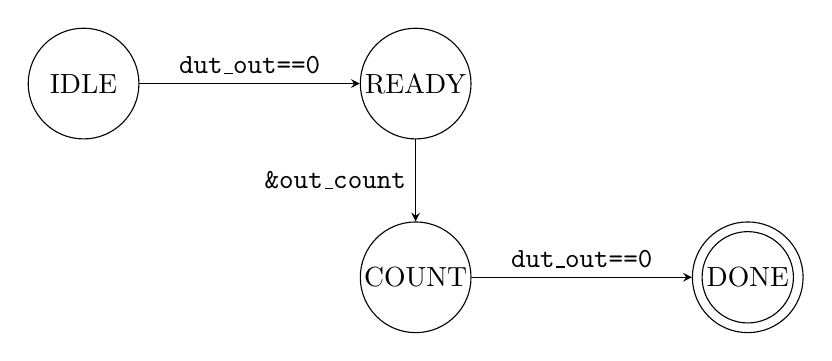
\begin{tikzpicture}
  [
    x=1em, y=1em,
    node/.style =
      {draw, circle, align=center, inner sep=0pt, minimum size=4em},
    sarrow/.style =
      { ->, >=stealth, font=\ttfamily}
  ]
  \node [node] at ( 0, 7)  (i) {IDLE};
  \node [node] at (12, 7) (r) {READY};
  \node [node] at (12, 0)  (c) {COUNT};
  \node [node] at (24, 0)  (d) {DONE};
  \node [draw, circle, inner sep=0pt, minimum size=3.3em] at (24, 0)  (dd) {};

  \draw [sarrow] (i.east)  -- node[above] {dut\_out==0}  (r.west);
  \draw [sarrow] (r.south) -- node[left]  {\&out\_count} (c.north);
  \draw [sarrow] (c.east)  -- node[above] {dut\_out==0}  (d.west);
\end{tikzpicture}
  \caption{Delay Tester FSM}
  \label{DelayTesterFSM}
\end{figure}

We first start a counter called \texttt{out\_count}.
Whenever this reaches all 1's, the driver output is set to some value with a known safe DUT output.
In this example, the safe output value is 0, which means when the delay tester is active, the driver will not generate any input to the DUT that will result in 0 on \texttt{dut\_out}.
The delay tester can then test the DUT delay with this safe value, since it knows when the DUT received the safe input, and can count the number of cycles until the DUT gives the safe output.

\begin{figure}[H]
  \centering
  \begin{tikztimingtable}
  [
    xscale=2.5,
    timing/d/background/.style={fill=white},
    timing/font=\ttfamily
  ]
  out\_count       & 6R 2{Q} 0R 8{Q} 0R 8{Q} 0R Q\\
                   & L 2{H 7L}       HL          \\
  o\_drive         & U 2{D{0} 7U}    D{0}U       \\
  i\_dut\_out      & U 2{3U D{0} 4U} 2U          \\
  test\_state      & 5D{00} 5D{01} 3D{10} 6D{11} \\
  delay\_out       & 11D{0} D{1} D{2} 6D{3}      \\
\extracode
  % Add vertical lines in two colors
  \begin{pgfonlayer}{background}
    \begin{scope}[semitransparent,semithick]
      \vertlines{1,2,...,18}
    \end{scope}
  \end{pgfonlayer}
\end{tikztimingtable}
  \caption{3-bit Delay Tester Waveform}
  \label{DelayTesterWF}
\end{figure}

The FSM starts in state IDLE.
When the first 0 output is detected from the DUT, the FSM enters the READY state.
It now knows that it can enter the COUNT state when the \texttt{out\_count} becomes all 1's again, triggering the next safe test input.
The FSM leaves the COUNT state for the DONE state when the safe output of 0 is detected.
The delay tester process is now complete and \texttt{out\_count} can be deactivated.

With this, the DUT's delay in clock cycles is the same as the number of cycles that the FSM stayed in state COUNT.
The delay counter \texttt{delay\_out} increments itself every cycle if the FSM is in that state.
When the FSM enters the DONE state, we the value of the delay counter is the delay of the DUT.
With a 3-bit counter as shown in the timing diagram, it can measure this delay for up to 8 clock cycles.
Longer delays can be measured by extending the width of \texttt{out\_count}.

\subsection{Limitations}
First, there has to be a safe value for the delay tester to use.
For adders and multipliers, this is relatively simple as LFSRs cannot generate zero as inputs and the output can only be zero if the both or one input is zero, respectively.
This is possible with subtracters as well since the two LFSRs will not produce the same number at the same time if they were seeded differently.
However, as soon as the ALU starts dealing with overflows, IEEE floating numbers, or any non-standard number representation system, there would be no guaranteed safe value without user input.
If the user have to input safe values for the delay tester to use, then if defeats the  purpose of saving one parameter for the user to configure.

The addition of this function also slowed down the $f_\text{max}$ to 315.06MHz.
As such, the idea of having an on-the-fly delay reconfiguration system was put on hold, as it might not be worth the engineering effort to save the user one single input.
